\newpage
\section{Formulación del problema}

\subsection{Descripción del problema}
Actualmente, la plataforma Paralegales presenta una serie de problemas estructurales derivados de decisiones técnicas tomadas durante su etapa inicial de desarrollo. Como se aprecia en la \autoref{fig:arbol_problemas}, el principal problema identificado es la exposición de lógica de negocio crítica en el cliente, lo que genera una serie de consecuencias negativas a nivel de seguridad, arquitectura, costos y gestión tecnológica.

Uno de los efectos más graves de esta exposición es el alto riesgo de inseguridad en la plataforma, ya que la lógica sensible puede ser inspeccionada, manipulada o replicada por terceros, lo que constituye un ejemplo de Insecure Design, una categoría de riesgo identificada en el OWASP Top 10 \cite{OWASP2021}.

Además, la dependencia de servicios propietarios como Firebase, fenómeno conocido como vendor lock-in \cite{OparaMartins2016, OparaMartins2014,Harauzek2022}, genera costos operativos más elevados y compromete la viabilidad económica de la plataforma a largo plazo. Asimismo, la falta de centralización en un único ecosistema tecnológico provoca fragmentación, lo que dificulta la integración, el mantenimiento y la escalabilidad del sistema.

Actualmente, Paralegales utiliza funciones AWS Lambda para manejar algunos casos de uso que requieren lógica crítica del lado del servidor. Sin embargo, mantener lógica crítica tanto en el frontend como en el backend (mediante Lambda) agrava la fragmentación tecnológica. Desde el punto de vista de diseño de sistemas (system design), esta dispersión de componentes críticos genera una arquitectura inconsistente y difícil de escalar y mantener, como se ilustra también en la \autoref{fig:arbol_problemas}.

En la raíz del problema, como se ilustra en la \autoref{fig:arbol_problemas}, se encuentra la priorización de la velocidad en el desarrollo sobre la adopción de buenas prácticas \cite{BirrEngwall2024}. Esta decisión condujo a una dependencia parcial de Firebase y sus tecnologías propietarias, así como a la omisión de delegar lógica crítica en entornos de ejecución que corren del lado del servidor como AWS Lambda o Cloud Functions, incrementando los riesgos mencionados.

Por lo tanto, se evidencia la necesidad urgente de una reestructuración tecnológica que permita resolver estos problemas, mejorando la seguridad, reduciendo costos, y garantizando una arquitectura sólida y escalable para el futuro del proyecto.

\begin{figure}[H]
  \centering
  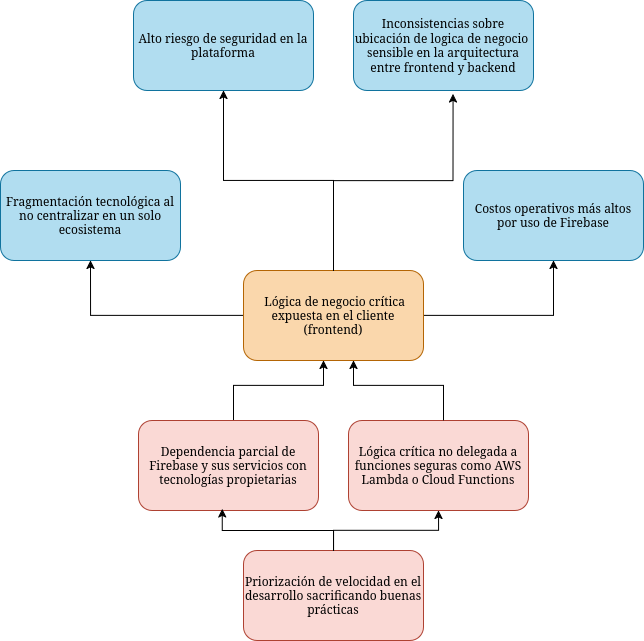
\includegraphics[width=0.85\textwidth]{img/figures/fig2-arbol-de-problemas.png}
  \caption{Árbol de problemas. Fuente: Elaboración Propia.}
  \label{fig:arbol_problemas}
\end{figure}

\subsection{Definición del Problema}
A partir del análisis realizado, se plantea como problema central a resolver el siguiente:
\begin{quote}
  \textbf{¿Cómo migrar y adaptar la infraestructura de la plataforma Paralegales desde Firebase hacia AWS de manera que se mejore la seguridad, se elimine la exposición de lógica crítica en el cliente, se reduzcan los costos operativos y se optimice la escalabilidad y mantenibilidad del sistema?}
\end{quote}

De este problema principal se derivan las siguientes preguntas específicas:

\begin{enumerate}
  \item \textbf{¿Qué servicios de AWS pueden reemplazar adecuadamente los servicios actuales de Firebase utilizados en Paralegales?}
  \item \textbf{¿Qué estrategias de migración permiten trasladar de forma segura y eficiente tanto los datos almacenados en la base de datos como los registros de usuarios desde Firebase hacia AWS, minimizando el impacto operativo?}
  \item \textbf{¿Cómo puede estructurarse una arquitectura basada en AWS que mejore la seguridad y reduzca la fragmentación tecnológica?}
  \item \textbf{¿Qué enfoques técnicos y metodológicos deben adoptarse durante el proceso de migración para garantizar la integridad de los datos y la continuidad del servicio?}
  \item \textbf{¿Qué medidas deben tomarse para optimizar los costos en AWS sin comprometer la calidad del servicio?}
\end{enumerate}

Estas preguntas guiarán el desarrollo del proyecto y permitirán estructurar un plan de migración que no solo atienda las necesidades actuales, sino que también prepare a la plataforma para un crecimiento seguro y sostenible.